\chapter{Design of Experimental Platform}\label{ch:platform}

This chapter presents the \ac{COTS} autopilots used in this research as well as outlining the Linux toolchain used to conduct |ac{SITL} and \ac{GCS} operations.  This chapter also introduces the airframes that were prototyped for testing specific performance characteristics discussed in Chapter~\ref{ch:performance}.

\section{Pixhawk Autopilot}
The Pixhawk autopilot is a collaborative project among open-source engineers which resulted in a high-performance autopilot which is capable of controlling aircraft, ground vehicles, and many others.  The primary reason this autopilot was chosen was because of the vast amount of support in the developer community.  The Pixhawk 1 autopilot hardware is effectively obsolete at the time of this writing, but the open-source code base is extremely flexible and continues to be ported to new hardware as it becomes available.  This has been the case for various Raspberry Pi autopilots as well as the Pixhawk 2.  The Pixhawk autopilot operates using two flight stacks (code base/operating systems); the PX4 flight stack and the \ac{APM} flight stack.  This research was implemented on the \ac{APM} flight stack primarily because the author's familiarity with the developer team which offers unparalleled assistance to the academic community.  The \ac{APM} codebase also offers a litany of open-source tools such as a Linux based \ac{GCS}, \ac{SITL} simulator, log analysis tools, and an \ac{API} for the RealFlight 7.5 simulator (high fidelity airframe simulation for small aircraft).

\begin{figure}[h!]
 \centering
  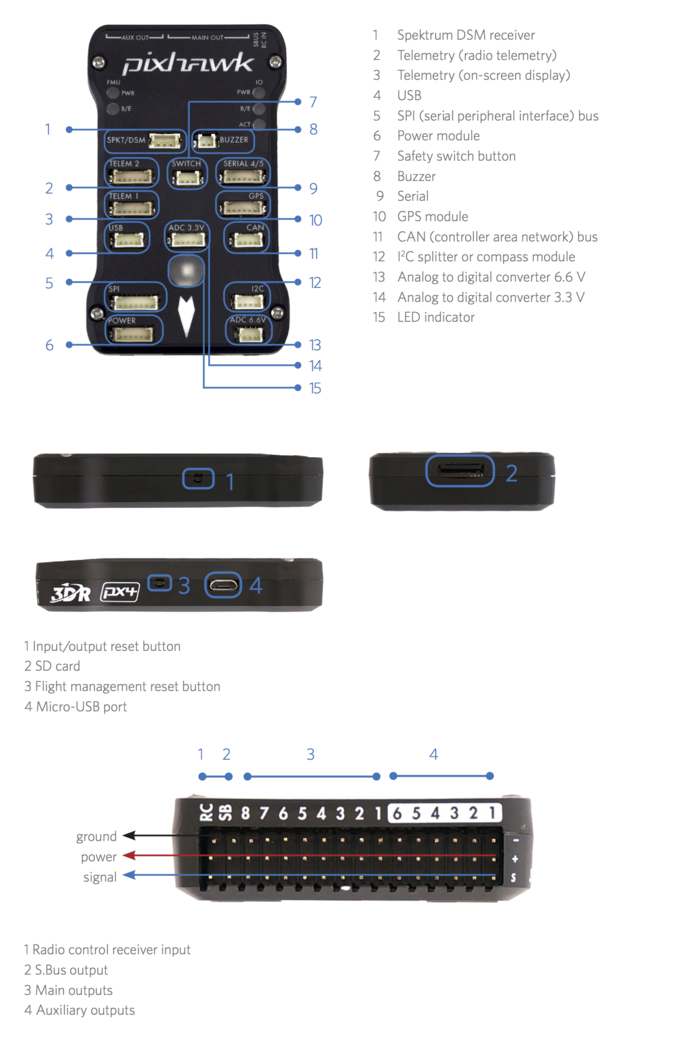
\includegraphics[width=0.65\textwidth]{pixhawk_connectors.png}
  \caption{Pixhawk 1 Autopilot Connection Diagram  \cite{apm_org}}
  \label{fig:pixhawk_autopilot}
\end{figure}

\subsection{Key Features}
The Pixhawk 1 Autopilot has the following features as found on \cite{apm_org}:
\begin{itemize}
\item 168 MHz / 252 MIPS Cortex-M4F
\item 14 PWM / Servo outputs (8 with failsafe and manual override, 6 auxiliary, high-power compatible)
\item Abundant connectivity options for additional peripherals (UART, I2C, CAN)
\item Integrated backup system for in-flight recovery and manual override with dedicated processor and stand-alone power supply (fixed-wing use)
\item Backup system integrates mixing, providing consistent autopilot and manual override mixing modes (fixed wing use)
\item Redundant power supply inputs and automatic failover
\item External safety switch
\item Multicolor LED main visual indicator
\item High-power, multi-tone piezo audio indicator
\item microSD card for high-rate logging over extended periods of time
\end{itemize}

\subsection{Specifications}
The Pixhawk 1 Autopilot has the following specifications as found on \cite{apm_org}:
\subsubsection{Processor}
\begin{itemize}
\item 32bit STM32F427 Cortex M4 core with FPU
\item 168 MHz
\item 256 KB RAM
\item 2 MB Flash
\item 32 bit STM32F103 failsafe co-processor
\end{itemize}
\subsubsection{Sensors}
\begin{itemize}
\item ST Micro L3GD20H 16 bit gyroscope
\item ST Micro LSM303D 14 bit accelerometer / magnetometer
\item Invensense MPU 6000 3-axis accelerometer/gyroscope
\item MEAS MS5611 barometer
\end{itemize}
\subsubsection{Interfaces}
\begin{itemize}
\item 5x UART (serial ports), one high-power capable, 2x with HW flow control
\item 2x CAN (one with internal 3.3V transceiver, one on expansion connector)
\item Spektrum DSM / DSM2 / DSM-X® Satellite compatible input
\item Futaba S.BUS® compatible input and output
\item PPM sum signal input
\item RSSI (PWM or voltage) input
\item I2C
\item SPI
\item 3.3 and 6.6V ADC inputs
\item Internal microUSB port and external microUSB port extension
\end{itemize}

\section{Ground Control Station}

The \ac{GCS} used for this research was MAVproxy \cite{mavproxy}.  It is an open-source python based \ac{GCS} which provides flexible communication and command with any autopilot utilizing the MAVlink protocol \cite{mavlink}.  Even though MAVproxy is written in Python (\ac{OS} agnostics language), it was found to be cumbersome to operate the \ac{GCS} on any other platform other than Linux.  This is primarily because the source code updates quite rapidly to support new features and the core developer (Andrew Tridgell) exclusively utilizes MAVproxy in Linux.  A significant amount of external libraries are utilized which results in a moderate amount of compatibility debugging for other \ac{OS}'s if desired.

\subsection{MAVproxy Features}
The following are summaries which proved to be extremely useful for this research \cite{mavproxy_wiki}:
\begin{itemize}
\item command-line, console based application. Plugins included in MAVProxy provide a basic \ac{GUI}.
\item network capable and run over any number of computers.
\item portable; capable of running on any POSIX OS with Python, pyserial, and select() function calls, which means Linux, OS X, Windows, and others.
\item light-weight design; runs on small netbooks.
\item tab-completion of commands.
\end{itemize}

\section{Simulation}
The \ac{APM} environment offers three versions of \ac{SITL} simulations.  The lowest fidelity \ac{SITL} is provided by MAVproxy, which is a simple 6-degree of freedom kinematics model with no environment or actuator modeling.  This proved to be adequate for initial testing but resulted in poorly tuned algorithms when actual flight tests were conducted.  The MAVproxy simulator was used for basic code debugging but nothing else.

The second \ac{SITL} offered in the \ac{APM} environment is X-plane 10.  This is a much higher fidelity simulation, which includes actuator models and environmental modeling.  X-plane 10 is primarily used for simulating full-scale aircraft and therefore is difficult to find models, which accurately represent the dynamics of small fixed-wing \ac{UAS}.  The open-source community provided model called the \enquote{maxi-swift} was similar enough to the airframe in this research that it provided adequate \ac{SITL} modeling which ensured robust flight test.

The last \ac{SITL} simulation tested under the \ac{APM} environment was the RealFlight 7.5 \ac{API}.  The RealFlight \ac{RC} airplane simulator offers some of the industry's highest fidelity simulations for small aircraft.  This product requires an \ac{API} key to hook into MAVproxy.  This capability is not yet on the market as of the time of this research, but the \ac{APM} core developers were supportive of this research and ran multiple experiments with the RealFlight \ac{SITL} for early validation.  The screenshot in Figure~\ref{fig:realflight_sitl} was captured while conducting testing utilizing the RealFlight \ac{SITL}.

\begin{figure}[h!]
 \centering
  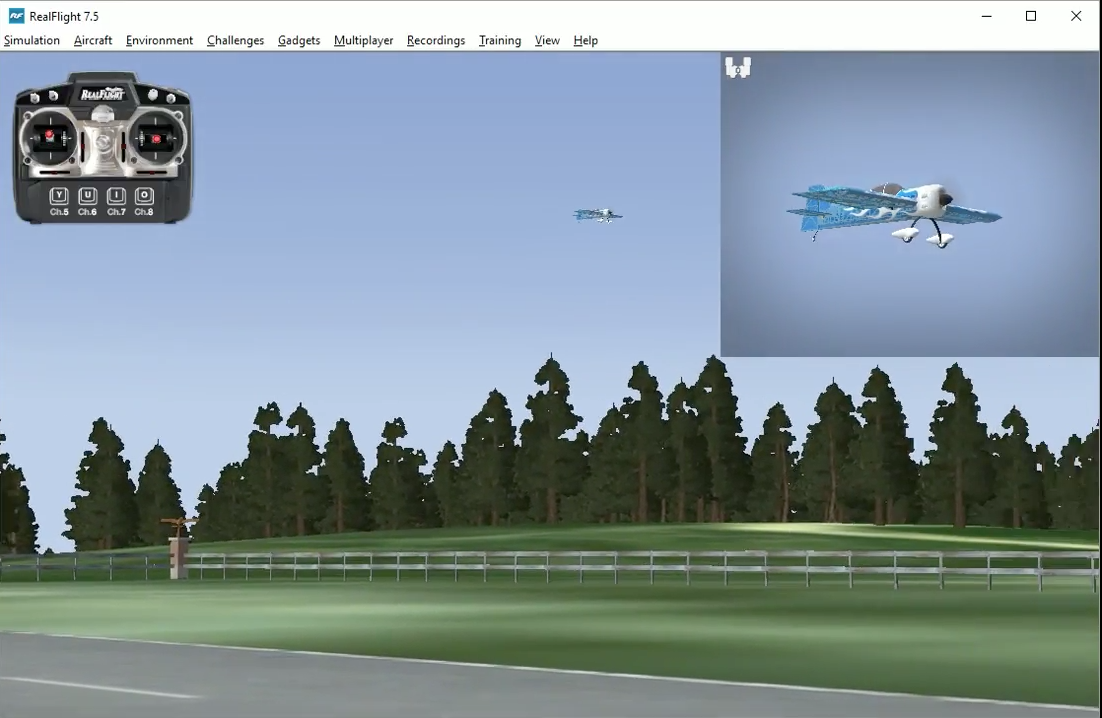
\includegraphics[width=0.65\textwidth]{realflight_simulator.png}
  \caption{High Fidelity RealFlight 7.5 \ac{SITL}}
  \label{fig:realflight_sitl}
\end{figure}


\section{Airframe}

The aircraft used for this research was the Flitetest Spear and the Flitetest Explorer \cite{flitetest}.  The Spear airframe was chosen for its endurance capability of greater than 45 minutes of flight time and its large capacity fuselage.  The flying-wing architecture keeps the actuation requirement to a minimum of two servos by utilizing an elevon configuration.

Figures~\ref{fig:spear} and \ref{fig:spear_carg} are example photos from the instructional build website \cite{flitetest}.

\begin{figure}[!h]
 \centering
  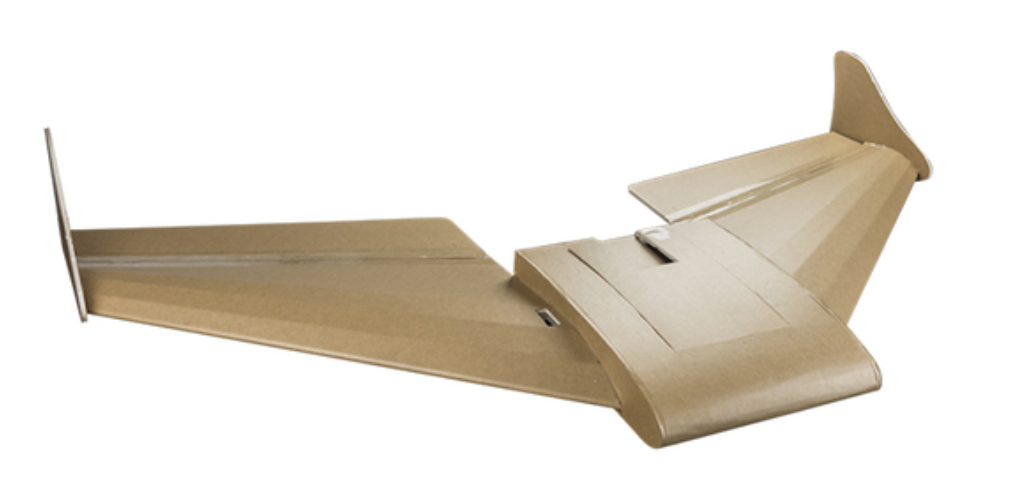
\includegraphics[width=0.65\textwidth]{spear.png}
  \caption{Spear Airframe \cite{flitetest}}
  \label{fig:spear}
\end{figure}

The large blunt nose provides adequate space for two 2,200 mAh (12.6volts) lithium polymer batteries wired in parallel.  The remaining cargo space was used for accommodating the Pixhawk autopilot.

\begin{figure}[!h]
 \centering
  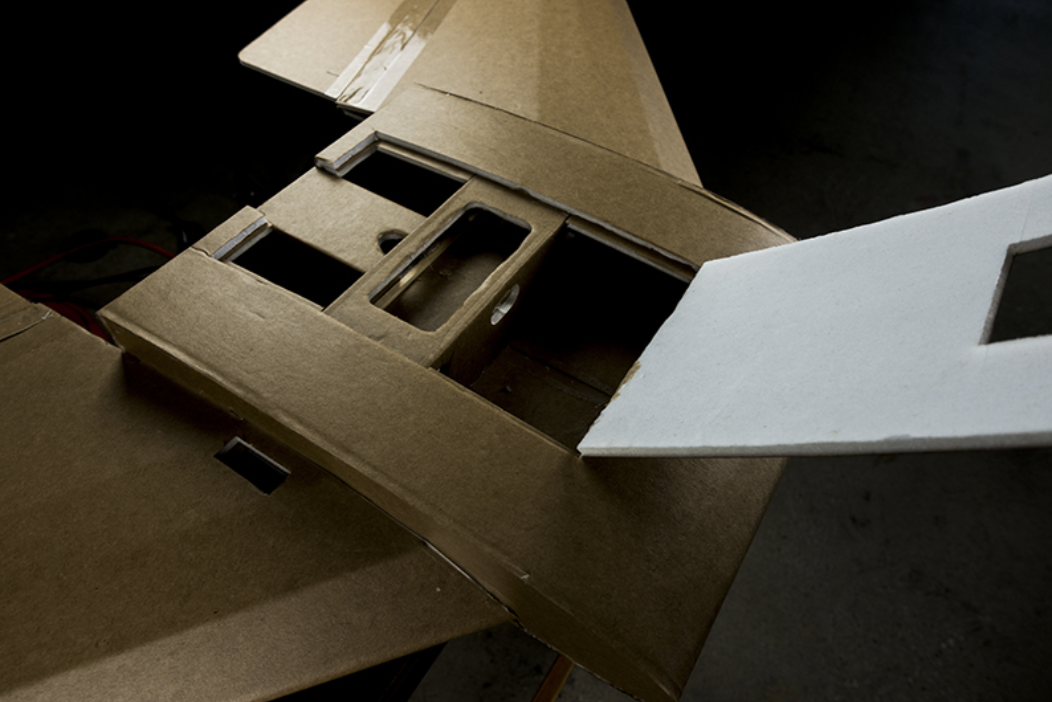
\includegraphics[width=0.6\textwidth]{spear_cargo.png}
  \caption{Spear Cargo Capacity \cite{flitetest}}
  \label{fig:spear_cargo}
\end{figure}

This plane was constructed out of craft foam board.  The plans were downloaded from flitetest.com\cite{flitetest} and converted to CorelDraw vector files for use in a laser cutter.  These files were then cut out of four sheets of foam board using the laser cutter.  The wing halves were joined with standard box tape and hot glue.  This provided a cheap and rapid construction process which was achievable under four hours of build time.

\begin{figure}[!h]
 \centering
  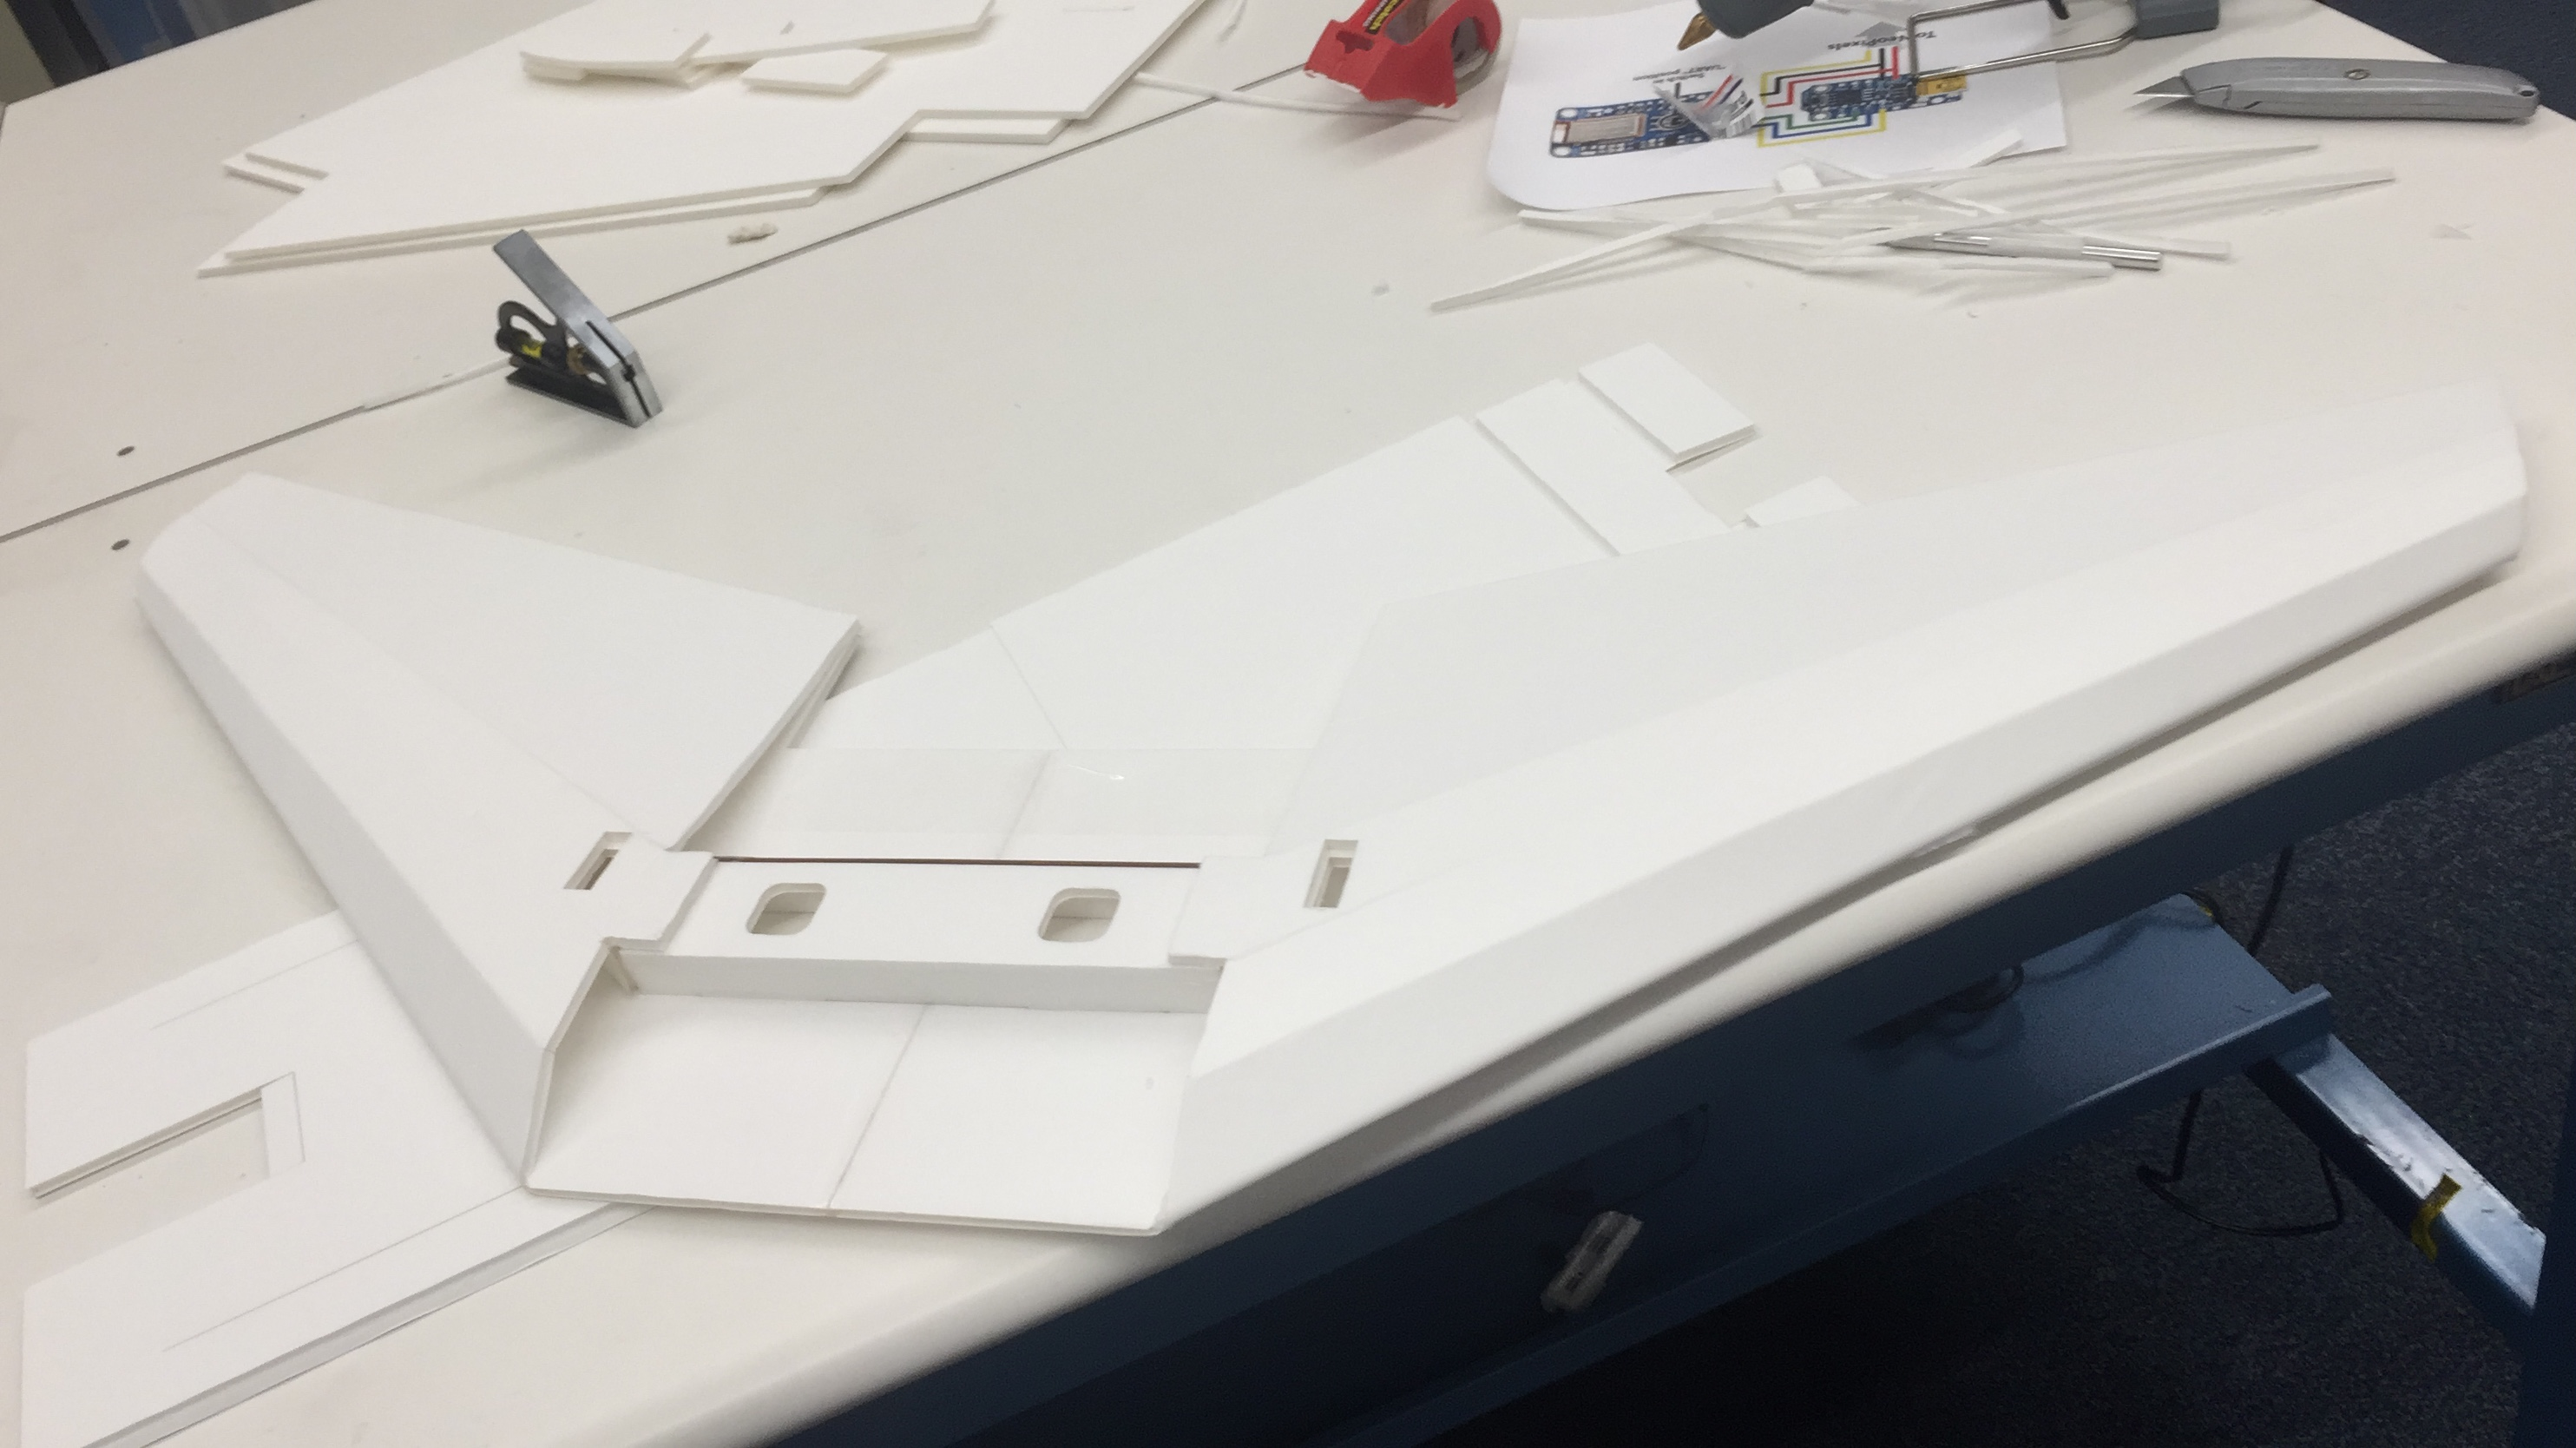
\includegraphics[width=0.6\textwidth]{spear_build.jpg}
  \caption{Spear Build Process}
  \label{fig:spear_build}
\end{figure}

\subsection{Spear Specifications}
\begin{itemize}
 \item weight without battery: 1.45 lbs (658 g)
 \item center of gravity: 3 – 3.5” (76 – 89 mm) in front of firewall
 \item control surface throws: 16\degrees  deflection – Expo 30\%
 \item wingspan: 41 inches (1041 mm)
 \item motor: 425 sized, 1200 kv minimum
 \item prop: 9 x 4.5 CW (reverse) prop
 \item electronic speed control (ESC): 30 amp minimum
 \item battery: (2) 2200 mAH 12.6 volt minimum
 \item xervos: (2) 9 gram servos 
\end{itemize}

The Explorer airframe was chosen because it is a conventional airframe with highly coupled aerodynamics which can be configured in multiple different failure modes.  The sport wing provided in the plans was modified to have independently actuated flaps, and ailerons for a combination of software enabled failure modes.  This aircraft was also configured with a rudder for testing the lateral aerodynamics coupling effects on the adaptive controller.  

\subsection{Explorer Specifications}
\begin{itemize}
 \item weight without battery: 1.08 lbs (493 g)
 \item center of gravity: 2.25” (57 mm) from leading edge of wing
 \item control surface throws: 12\degrees  deflection – Expo 30\%
 \item wingspan: 57 inches (1447 mm)
 \item motor: 425 sized, 1000 kv minimum
 \item prop: 9 x 6 CW (reverse) prop
 \item ESC: 30 amp minimum
 \item battery: (1) 2200 mAH 12.6 volt minimum
 \item servos: (6) 9 gram servos 
\end{itemize}

\begin{figure}[!h]
 \centering
  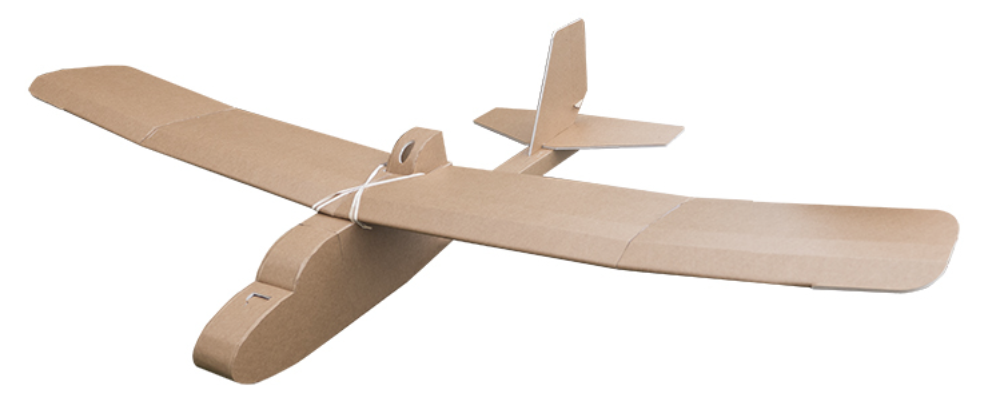
\includegraphics[width=0.90\textwidth]{explorer.png}
  \caption{FliteTest Explorer \cite{flitetest}}
  \label{fig:explorer_parts}
\end{figure}

\begin{figure}[!h]
 \centering
  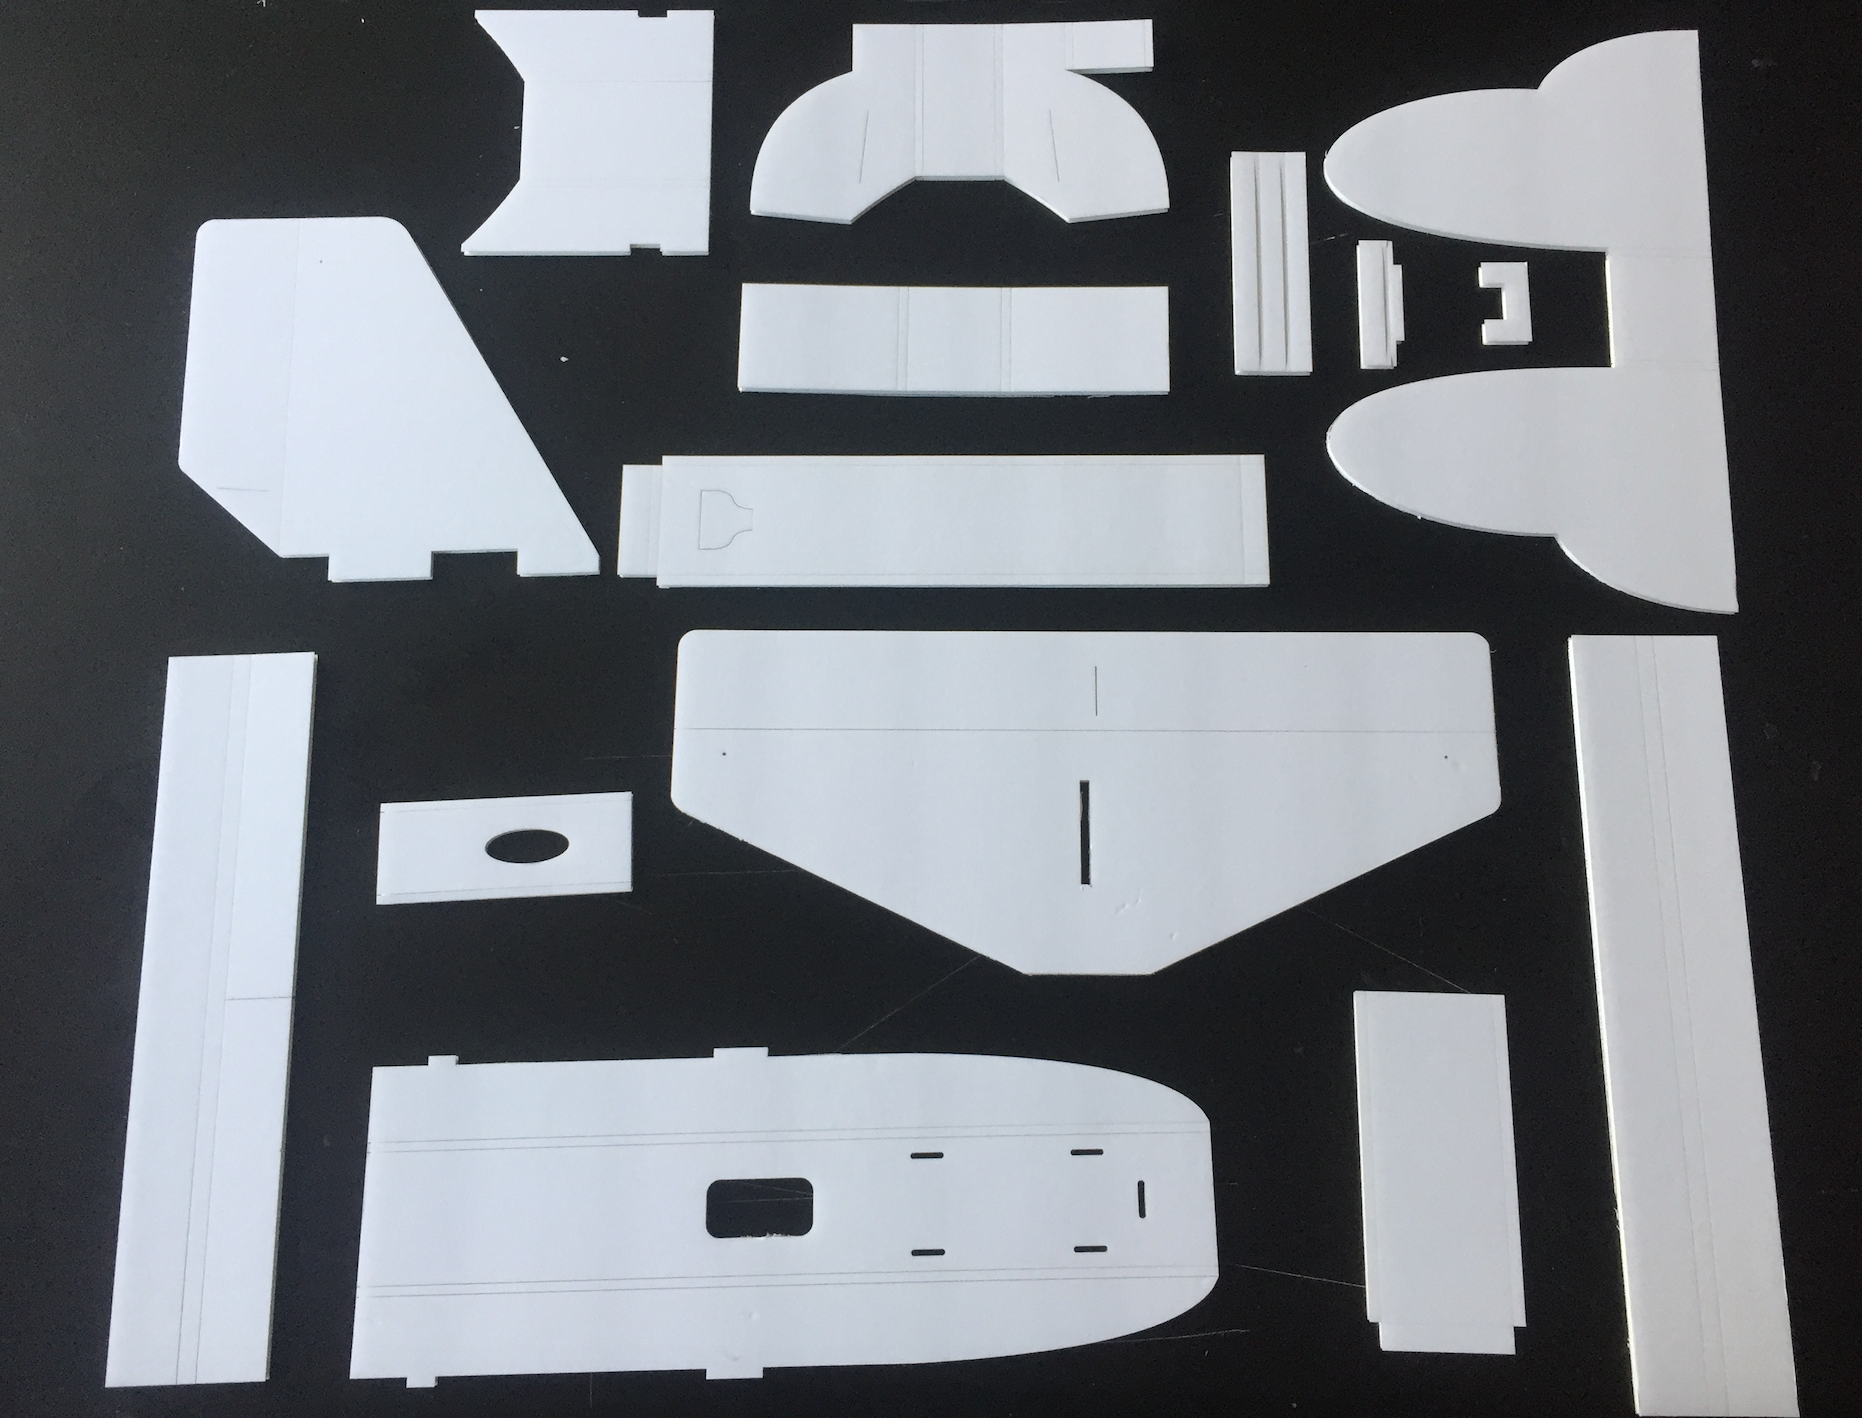
\includegraphics[width=0.85\textwidth]{explorer_parts.png}
  \caption{Explorer Cut Foamboard Parts}
  \label{fig:explorer_parts}
\end{figure}

\begin{figure}[!h]
 \centering
  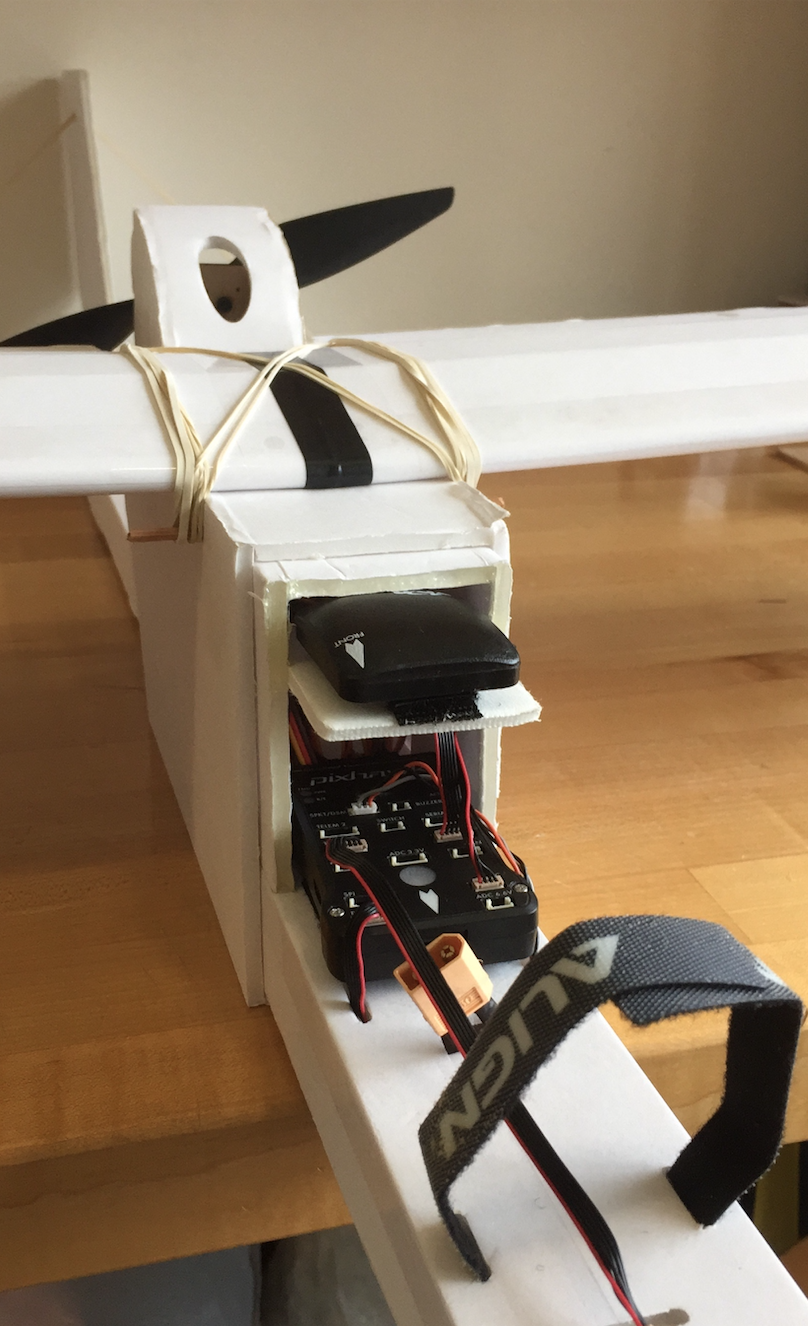
\includegraphics[width=0.75\textwidth]{explorer_electronics.png}
  \caption{Pixhawk Autopilot Installed on Explorer}
  \label{fig:explorer_electronics}
\end{figure}

The previously discussed \ac{COTS} autopilot, Linux software tool chain for \ac{SITL} and \ac{GCS}, and prototype aircraft were utilized to present the results found in Chapter~\ref{ch:performance}.



